
\chapter{CONFIGURACIÓN EXPERIMENTAL}

En esta sección se presenta la configuración experimental sobre las simulaciones
realizadas con el fin de validar la efectividad del algoritmo desarrollado, realizando una
descripción de los conjuntos de datos usados para la validación, las métricas escogidas, y
los algoritmos del estado del arte para la comparación.

\section{CONJUNTO DE DATOS}

Se dispone de un extenso conjunto de datos compuesto por imágenes de retina de alta
resolución, tomadas bajo diversas condiciones de imagen. Cada sujeto tiene asignados
campos para el ojo izquierdo y derecho, identificados con el número de paciente seguido de
"izquierda" o "derecha" (por ejemplo, 1\_izquierda.jpeg es el ojo izquierdo del paciente
con identificación 1).Cada imagen fue evaluada por un clínico para determinar la presencia
de retinopatía diabética, utilizando una escala de 0 a 4 que indica la gravedad de la
condición. Esta escala incluye los siguientes niveles: 0 (sin retinopatía diabética), 1
(leve), 2 (moderada), 3 (severa) y 4 (retinopatía diabética proliferativa).

Las imágenes en el conjunto de datos provienen de diversas cámaras y modelos, lo que puede
afectar la apariencia visual de las imágenes izquierdas y derechas. Algunas imágenes
presentan la anatomía de la retina de manera convencional, con la mácula a la izquierda y
el nervio óptico a la derecha para el ojo derecho. Otras imágenes muestran una vista
invertida, como se observaría a través de una lente de microscopio durante un examen
ocular en vivo. Identificar si una imagen está invertida se basa en dos criterios: la
posición relativa de la mácula con respecto al nervio óptico y la presencia de una muesca
en el lateral de la imagen.

Es importante tener en cuenta que tanto las imágenes como las etiquetas pueden contener
ruido, como artefactos, desenfoque, subexposición o sobreexposición. Por lo tanto, nuestro
objetivo principal es desarrollar algoritmos robustos capaces de funcionar en condiciones
de ruido y variabilidad.

\subsection{DESCRIPCIÓN DEL DATASET}

Se dispone de un extenso conjunto de datos compuesto por imágenes de retina de alta
resolución, tomadas bajo diversas condiciones de imagen. Cada sujeto tiene asignados
campos para el ojo izquierdo y derecho, identificados con el número de paciente seguido de
“izquierda” o "derecha" (por ejemplo, 1\_izquierda.jpeg es el ojo izquierdo del paciente
con identificación 1). Cada imagen fue evaluada por un clínico para determinar la
presencia de retinopatía diabética, utilizando una escala de 0 a 4 que indica la gravedad
de la condición. Esta escala incluye los siguientes niveles: 0 (sin retinopatía
diabética), 1 (leve), 2 (moderada), 3 (severa) y 4 (retinopatía diabética proliferativa).


\begin{figure}[H]
    \centering
    \caption{muestra del dataset}
    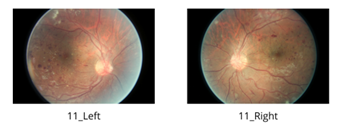
\includegraphics[width=1\textwidth]{imágenes/conf_exp/derecho-izquierdo.png} 
    \caption*{\textit{Fuente: }} 
\end{figure}

Las imágenes en el conjunto de datos provienen de diversas cámaras y modelos, lo que puede
afectar la apariencia visual de las imágenes izquierdas y derechas. Algunas imágenes
presentan la anatomía de la retina de manera convencional, con la mácula a la izquierda y
el nervio óptico a la derecha para el ojo derecho. Otras imágenes muestran una vista
invertida, como se observaría a través de una lente de microscopio durante un examen
ocular en vivo. Identificar si una imagen está invertida se basa en dos criterios: la
posición relativa de la mácula con respecto al nervio óptico y la presencia de una muesca
en el lateral de la imagen. Es importante tener en cuenta que tanto las imágenes como las
etiquetas pueden contener ruido, como artefactos, desenfoque, subexposición o
sobreexposición. Por lo tanto, nuestro objetivo principal es desarrollar algoritmos
robustos capaces de funcionar en condiciones de ruido y variabilidad. Los datos utilizados
para este estudio se han tomado de Diabetic Retinopathy Detection 2015 y APTOS 2019
blindness detection de kaggle. Ambos conjuntos de datos contienen miles de imágenes de
retina bajo diferentes condiciones.



\section{MÉTRICAS DE EVALUACIÓN}

En los estudios de clasificación médica, existen diferentes cálculos de medidas de
desempeño ampliamente utilizados. La precisión, la sensibilidad y la especificidad son
algunos de ellos, y estas medidas se emplean para evaluar la precisión de un método
utilizado. Las ecuaciones utilizadas para calcular estas medidas son las siguientes:



\vskip 1em

En las anteriores ecuaciones, TP y FP se utilizan para definir el número de diagnósticos
verdaderos positivos y el número de diagnósticos falsos positivos. Por otro lado, TN y FN
son para el número de diagnósticos verdaderos negativos y el número de diagnósticos falsos
negativos. N es el número de muestras totales, lo que significa también la suma de
muestras positivas y negativas en el proceso de clasificación.

Para un problema de clasificación, la capacidad de diagnosticar correctamente se calcula a
través de la precisión. Además, la tasa de sensibilidad define el grado en el que el
modelo define correctamente la clase objetivo. Por otro lado, la tasa de precisión es para
comprender cómo el clasificador proporciona cierta determinación de clase. Finalmente, el
valor Fscore es una media armónica de la precisión y la sensibilidad para entender mejor
ambas capacidades con un valor. En este estudio, todos los parámetros de evaluación
relacionados se utilizaron para probar el rendimiento del enfoque de solución a través de
diferentes perspectivas requeridas.

\section{ENTORNO DE DESARROLLO Y HERRAMIENTAS}

\subsection{LENGUAJE DE PROGRAMACIÓN}

En el desarrollo de este trabajo de investigación, se consideraron algunos lenguajes de
programación para la implementación de las CNNs cada uno con aspectos particulares en el
ámbito del procesamiento de imágenes y el aprendizaje profundo. En primer lugar se tomo en
cuenta R, un lenguaje con una gran variedad de paquetes especializados en modelos
estadísticos y aprendizaje automático. Sin embargo, su desempeño en tareas de deep
learning es limitado en comparación con otros lenguajes como C++, un lenguaje altamente
eficiente y optimizado, utilizado en aplicaciones donde el rendimiento es crítico. No
obstante, su curva de aprendizaje es más pronunciada y el desarrollo de modelos de
aprendizaje profundo en este lenguaje requiere una mayor cantidad de código en comparación
con lenguajes de alto nivel. De este modo, se optó por Python debido a su sintaxis clara y
legible que facilita la implementación de modelos complejos. Además, cuenta con una amplia
comunidad de desarrolladores y científicos que contribuyen con documentación, foros de
discusión y soluciones a problemas frecuentes, lo que resulta en un entorno de desarrollo
altamente colaborativo. Python cuenta con un ecosistema robusto de herramientas,
incluyendo librerías como NumPy, Pandas y Matplotlib, que son fundamentales para la
manipulación y análisis de datos, así como para la visualización de resultados. Asimismo,
su compatibilidad con aceleradores de hardware, como GPUs y TPUs, permite el entrenamiento
eficiente de modelos a gran escala, reduciendo significativamente el tiempo de cómputo
requerido.

\subsection{ENTORNO DE DESARROLLO INTEGRADO(IDE)}

Se evaluaron distintos entornos de desarrollo integrados (IDE) donde cada uno ofrece
ventajas y características específicas que pueden influir en la ejecución de los modelos.
Uno de ellos es Jupyter Notebook, una herramienta ampliamente utilizada en investigación y
desarrollo de proyectos de ciencia de datos debido a su flexibilidad y capacidad para
ejecutar código de manera interactiva. Sin embargo, su uso requiere una configuración
manual del entorno y la disponibilidad de recursos computacionales locales. Google Colab,
en cambio, es una opción muy utilizada para el desarrollo en la nube, ya que proporciona
acceso gratuito a GPUs/TPUS y facilita la colaboración en tiempo real. No obstante,
presenta ciertas limitaciones en cuanto a la estabilidad de las sesiones, acceder a una de
sus GPUs gratuitas es difícil debido a la alta demanda, y el entorno se desconecta con
frecuencia, lo que interrumpe el flujo de trabajo. En definitiva, se seleccionó los
notebooks en la nube de Kaggle para la implementación debido a su estabilidad y a la
posibilidad de activar una GPU en cualquier momento, con un límite de uso de 30 horas
semanales. Esta plataforma proporciona una GPU NVIDIA Tesla P100 con 16 GB de memoria,
además de la opción de utilizar una NVIDIA T4 x2. Este hardware de alto rendimiento
optimiza las tareas de aprendizaje automático, agilizando tanto el entrenamiento de
modelos como la inferencia.

\subsection{FRAMEWORKS}

Se seleccionó TensorFlow junto con su API de alto nivel Keras como framework principal,
esta decisión se basó principalmente en que Tensorflow cuenta con una amplia adopción en
el ámbito clínico y de investigación biomédica, ofreciendo herramientas probadas para el
procesamiento de imágenes médicas \myfootcite{stanescu2023tensorflow}. Su integración con
Keras simplifica la implementación de arquitecturas complejas (p. ej., ResNet,
EfficientNet) mientras mantiene robustez en entornos productivos. Proporciona un
rendimiento eficiente en entornos con GPUs limitadas (como las ofrecidas por Kaggle: Tesla
P100/T4), gracias a optimizaciones integradas (XLA, Grappler). Keras ofrece acceso directo
a modelos preentrenados en TensorFlow Hub, ajustables para clasificación multiclase de
retinopatía. Además, su ecosistema facilita el despliegue en clínicas mediante TensorFlow
Lite o TF Serving, crucial para una futura implementación en entornos hospitalarios. La
suite TensorFlow Extended incluye módulos para aumento de datos (tf.image) y
preprocesamiento de imágenes médicas (normalización de histogramas, ajuste de contraste),
esenciales para abordar variabilidad en las imágenes de fondo de ojo (iluminación,
artefactos). Si bien PyTorch es destacable por su flexibilidad en investigación
experimental requiere más desarrollo manual para estas tareas, TensorFlow/Keras demostró
mayores ventajas en este proyecto al equilibrar productividad, eficiencia computacional y
facilidad de integración.

\section{CONFIGURACIÓN EXPERIMENTAL EN CLASIFICADOR MULTICLASE}

Para esta investigación se mantuvo un marco experimental común tanto para el clasificador
binario como para el multiclase, utilizando las mismas herramientas principales: el
lenguaje de programación Python, la biblioteca TensorFlow y el entorno de desarrollo
provisto por Kaggle. Sin embargo, algunas configuraciones específicas difieren entre ambos
enfoques, particularmente en el tratamiento de los datos antes del entrenamiento, la
selección de ciertos hiperparámetros y la configuración del acelerador dentro del entorno
de Kaggle.

Además, el objetivo del clasificador multiclase introduce una variación importante en el
enfoque experimental. Si bien, al igual que el clasificador binario, busca obtener
resultados óptimos y confiables para su eventual aplicación en un contexto médico, este
modelo también tiene como propósito comparar el desempeño del sistema al procesar imágenes
bajo distintos canales de color (rojo, verde, azul) y en su versión RGB estándar, además
se utilizo la tecnica de ajuste fino para ver como varía el desempeño de cada modelo
planteado segun su artitectura. De esta forma, se pretende determinar bajo qué condiciones
el modelo multiclase alcanza un rendimiento superior, lo cual puede aportar información
relevante sobre la influencia del preprocesamiento visual en la detección de retinopatía
diabética.

\subsection{TRATAMIENTO DE DATOS}

Durante el análisis exhaustivo del conjunto de datos, se identificaron varios problemas
que afectan negativamente el desempeño de los modelos de clasificación multiclase. Entre
los principales desafíos se encontraron una cantidad significativa de imágenes dañadas o
de baja calidad, las cuales dificultan el proceso de aprendizaje del modelo, así como un
notable desbalance entre las clases, especialmente por la predominancia de la clase
correspondiente a pacientes sanos. Este desbalance puede llevar al modelo a sesgar sus
predicciones hacia la clase mayoritaria, reduciendo su capacidad de generalización. Por
ello, fue necesario aplicar estrategias específicas de limpieza, filtrado y balanceo,
orientadas a mejorar la calidad de los datos sin eliminar muestras valiosas ni conservar
imágenes que pudieran perjudicar el entrenamiento.

\subsubsection{LIMPIEZA GENERAL DEL DATASET}

Durante el proceso de exploración y limpieza del conjunto de datos, se identificó un
número considerable de imágenes que presentaban problemas severos de iluminación: algunas
eran casi completamente oscuras y otras excesivamente brillantes. En ambas situaciones
resultaba imposible distinguir adecuadamente la circunferencia del globo ocular o las
estructuras internas relevantes para la detección de retinopatía diabética. A pesar de
ello, estas imágenes estaban etiquetadas con niveles de severidad entre 0 y 4, lo que
indicaba que habían sido consideradas válidas en el conjunto original. No obstante, su
falta de información visual útil no solo limita su valor diagnóstico, sino que también
puede introducir ruido y dificultar el proceso de aprendizaje del modelo.

Para abordar este problema, se diseñó un procedimiento automático de limpieza basado en el
análisis del brillo promedio de las imágenes. Esta estrategia consistió en convertir cada
imagen a escala de grises y calcular su luminosidad media. Si el valor promedio se
encontraba por debajo de un umbral establecido para imágenes demasiado oscuras o por
encima de un umbral para imágenes excesivamente brillantes, la imagen se consideraba no
apta para el entrenamiento. Aquellas que cumplían con estos criterios eran automáticamente
separadas del conjunto principal y movidas a una carpeta de exclusión. Este proceso se
implementó utilizando OpenCV y NumPy en Python, y permitió filtrar de manera eficiente las
imágenes que no aportan información significativa al modelo de clasificación multiclase.

\subsection{BALANCEO DE CLASES}

El conjunto de datos original presenta un marcado desbalance entre las clases, lo cual
representa un desafío importante para la construcción de un clasificador multiclase
efectivo. En particular, la clase 0 correspondiente a pacientes sanos representa
aproximadamente el 73\% del total de muestras, mientras que la clase 4 asociada a la
retinopatía diabética proliferativa, la forma más severa de la enfermedad, apenas alcanza
el 2\% . Esta relación superior a 4:1 entre la clase mayoritaria y la minoritaria tiende a
sesgar el aprendizaje del modelo\myfootcite{johnson2019survey}, disminuyendo su capacidad
para detectar correctamente las clases menos representadas, como se evidenció en pruebas
previas.

Para mitigar este desbalance, se implementó una estrategia de balanceo que consistió en
reducir el número de muestras de la clase 0 y aumentar artificialmente las muestras de las
clases con menor representación. Sin embargo, una reducción aleatoria directa del volumen
de la clase 0 no ofreció los resultados esperados. Un análisis más detallado reveló que
esta clase contenía una alta proporción de imágenes con ruido o calidad cuestionable, lo
que implicaba el riesgo de eliminar muestras útiles y conservar otras potencialmente
perjudiciales para el entrenamiento. Por esta razón, antes de aplicar la reducción
aleatoria, se realizó una limpieza manual de la clase 0 con el fin de preservar las
imágenes más relevantes y eliminar aquellas que pudieran afectar negativamente el
desempeño del modelo. Esta etapa permitió establecer una base más sólida para alcanzar un
equilibrio adecuado en el conjunto de datos multiclase.

\subsubsection{FILTRADO CLASE 0}

En el proceso de limpieza de la clase 0, se identificaron y eliminaron aquellas imágenes
que contenían ruido significativo en la región del ojo, utilizando un enfoque basado en el
procesamiento de imágenes. Cada imagen fue primero convertida a escala de grises para
simplificar el análisis de luminosidad y contraste. Posteriormente, se aplicó el operador
de Canny para detectar los bordes, un paso inicial para identificar estructuras en la
imagen, posteriormente se utilizó la Transformada de Hough para círculos con el fin de
localizar la principal estructura circular dentro de la imagen,la cual corresponde al ojo.
Esto permitió enfocar el análisis de ruido exclusivamente en la región de interés, a
través de umbrales de brillo se busco contornos lo suficientemente grandes para ser
considerados como ruidos y no

\subsubsection{AUMENTO DE DATOS}

El aumento de datos, aunque es una técnica común y poderosa dentro del aprendizaje
profundo, debe ser aplicado con cautela, especialmente cuando se trabaja con modelos
preentrenados. Estos modelos, al contar con una gran cantidad de parámetros ajustables,
pueden ser más propensos al sobreajuste si se les expone a transformaciones que alteran
excesivamente la naturaleza de los datos originales.

Para mitigar este riesgo, se priorizó el uso de transformaciones que introducen
variabilidad sin modificar la estructura fundamental de la imagen. Estas técnicas
preservan la integridad visual de las retinografías al tiempo que enriquecen la diversidad
del conjunto de entrenamiento \myfootcite{shorten2019survey}. Entre las transformaciones
más efectivas y menos invasivas se encuentran las alteraciones geométricas simples, los
ajustes de brillo o color, la introducción de ruido controlado y las técnicas de mezcla
como el mixup o cutmix. En este caso específico, se implementó un conjunto de
transformaciones geométricas moderadas utilizando la clase ImageDataGenerator de Keras,
que permitió generar nuevas muestras a partir de imágenes existentes de forma controlada.
Las transformaciones incluyeron rotaciones aleatorias de hasta 10 grados, zoom aleatorio
de hasta un 5\% , desplazamientos horizontales y verticales leves, volteo horizontal de
las imágenes, relleno con interpolación para preservar bordes y evitar errores visuales
durante las transformaciones. Estas operaciones fueron aplicadas únicamente a las clases
minoritarias (1,2,3,4) con el objetivo de equilibrar la distribución del conjunto de
datos.


Al concluir los procesos de limpieza y aumento de datos, obtenemos un conjunto de datos
significativamente más robusto, con menos información que pudiera interferir con el
aprendizaje del modelo. Además, se ha logrado un balance adecuado entre las clases, lo que
favorece una mayor capacidad de generalización en el modelo. El dataset resultante,
optimizado y equilibrado, tiene la siguiente distribución:



\subsection{ARQUITECTURA DEL MODELO MULTICLASE}

Para el experimento del clasificador multiclase, se emplearon cuatro arquitecturas base
pre-entrenadas en ImageNet y ampliamente utilizadas en el dominio médico: ResNet50V2,
InceptionV3, VGG19 y MobileNetV2. Sobre cada una de estas bases, se diseñaron dos
configuraciones de capas densas (“top model”). La primera configuración consistió en dos
capas densas de 512 y 256 unidades con activación ReLU; la segunda empleó una estructura
más ligera, de 256 y 128 unidades, igualmente con activación ReLU. En ambos casos, la capa
de salida fue una densa con cinco neuronas y activación softmax, correspondiente a las
cinco clases del problema.
Estas configuraciones , 512-256 y 256→128 se encuentran entre las más utilizadas en la
literatura para tareas similares. Por ejemplo, un estudio reciente sobre diagnóstico de
retinopatía diabética utilizando redes densamente conectadas (DenseNet121) empleó capas
densas de 256 y 128 unidades después del extractor convolutional biomed.bas.bg. No
obstante, se han reportado configuraciones alternativas que no se explorarán en este
proyecto. En particular, un trabajo que utilizó la arquitectura Xception propuso un “top
model” compuesto por cinco capas densas con 1024, 256, 128, 64 y 32 unidades
ScienceDirect. En general, las variantes con bloques densos que contienen 256 y 128 0 512
y 256 unidades aparecen de forma recurrente en estudios de DR con fine-tuning parcial o
cabezales personalizados, lo que respalda su selección en este trabajo.MDPI+1
Todas las capas convolucionales de cada red base fueron congeladas durante esta fase de
experimentación, permitiendo entrenar únicamente las capas densas superiores. Esto
facilitó evaluar la capacidad de transferencia de características desde el dominio general
de ImageNet al dominio específico de imágenes médicas, con un entrenamiento rápido y
controlado.
El entrenamiento se realizó durante tres épocas, sin aplicar técnicas adicionales de
regularización como dropout o early stopping, dado que el propósito fue comparar el
comportamiento básico de cada arquitectura bajo condiciones homogéneas. Se utilizó el
optimizador Adam y la función de pérdida sparse categorical crossentropy, adecuada para
clasificación multiclase con etiquetas en formato entero.
Al concluir el entrenamiento, los modelos fueron evaluados tanto en el conjunto de
entrenamiento como en el de validación. Se generaron métricas clave —precisión
(precision), recuperación (recall), puntuación F1 (F1-score) y exactitud (accuracy)—
mediante el informe de clasificación de scikit-learn. Los resultados se almacenaron y
organizaron para su análisis comparativo. Además, se elaboraron gráficos que muestran la
evolución de la pérdida y exactitud durante el entrenamiento, lo que permitió observar
visualmente el rendimiento diferencial de cada arquitectura.

Para la elección de la configuración aunque se tuvo en cuenta todas las métricas se
intentó dar un mayor énfasis sobre la sensibilidad (recall) , métrica que suele ser unas
de las más relevantes para estudios médicos. La configuración 256–128 supera a 512–256 no
solo en sensibilidad media, sino también, ligeramente, en precisión media , F1 medio y
exactitud media. Asimismo, tres de las cuatro arquitecturas base (ResNet50V2, MobileNetV2,
InceptionV3) alcanzaron su mejor recall en validación con 256–128; la excepción fue VGG19,
cuyo mejor resultado se dio con 512–256.
